\paragraph{V1 - Python}
Die Pythonversion ist basierend auf einem Queue System, bei dem verschiedene Komponenten in verschiedenen \Glspl{thread} selbstständig Jobs und Events hinzufügen können. Ein oder mehrere Job-Handler sollen sich anschließend Jobs aus der Queue entnehmen und ausführen. Ein Job-Handler sollte eine Einlagerungsstation darstellen, somit sollten meherere verschiedene Auslagerungsstationen abgebildet werden können.

\begin{figure}
  \centering
  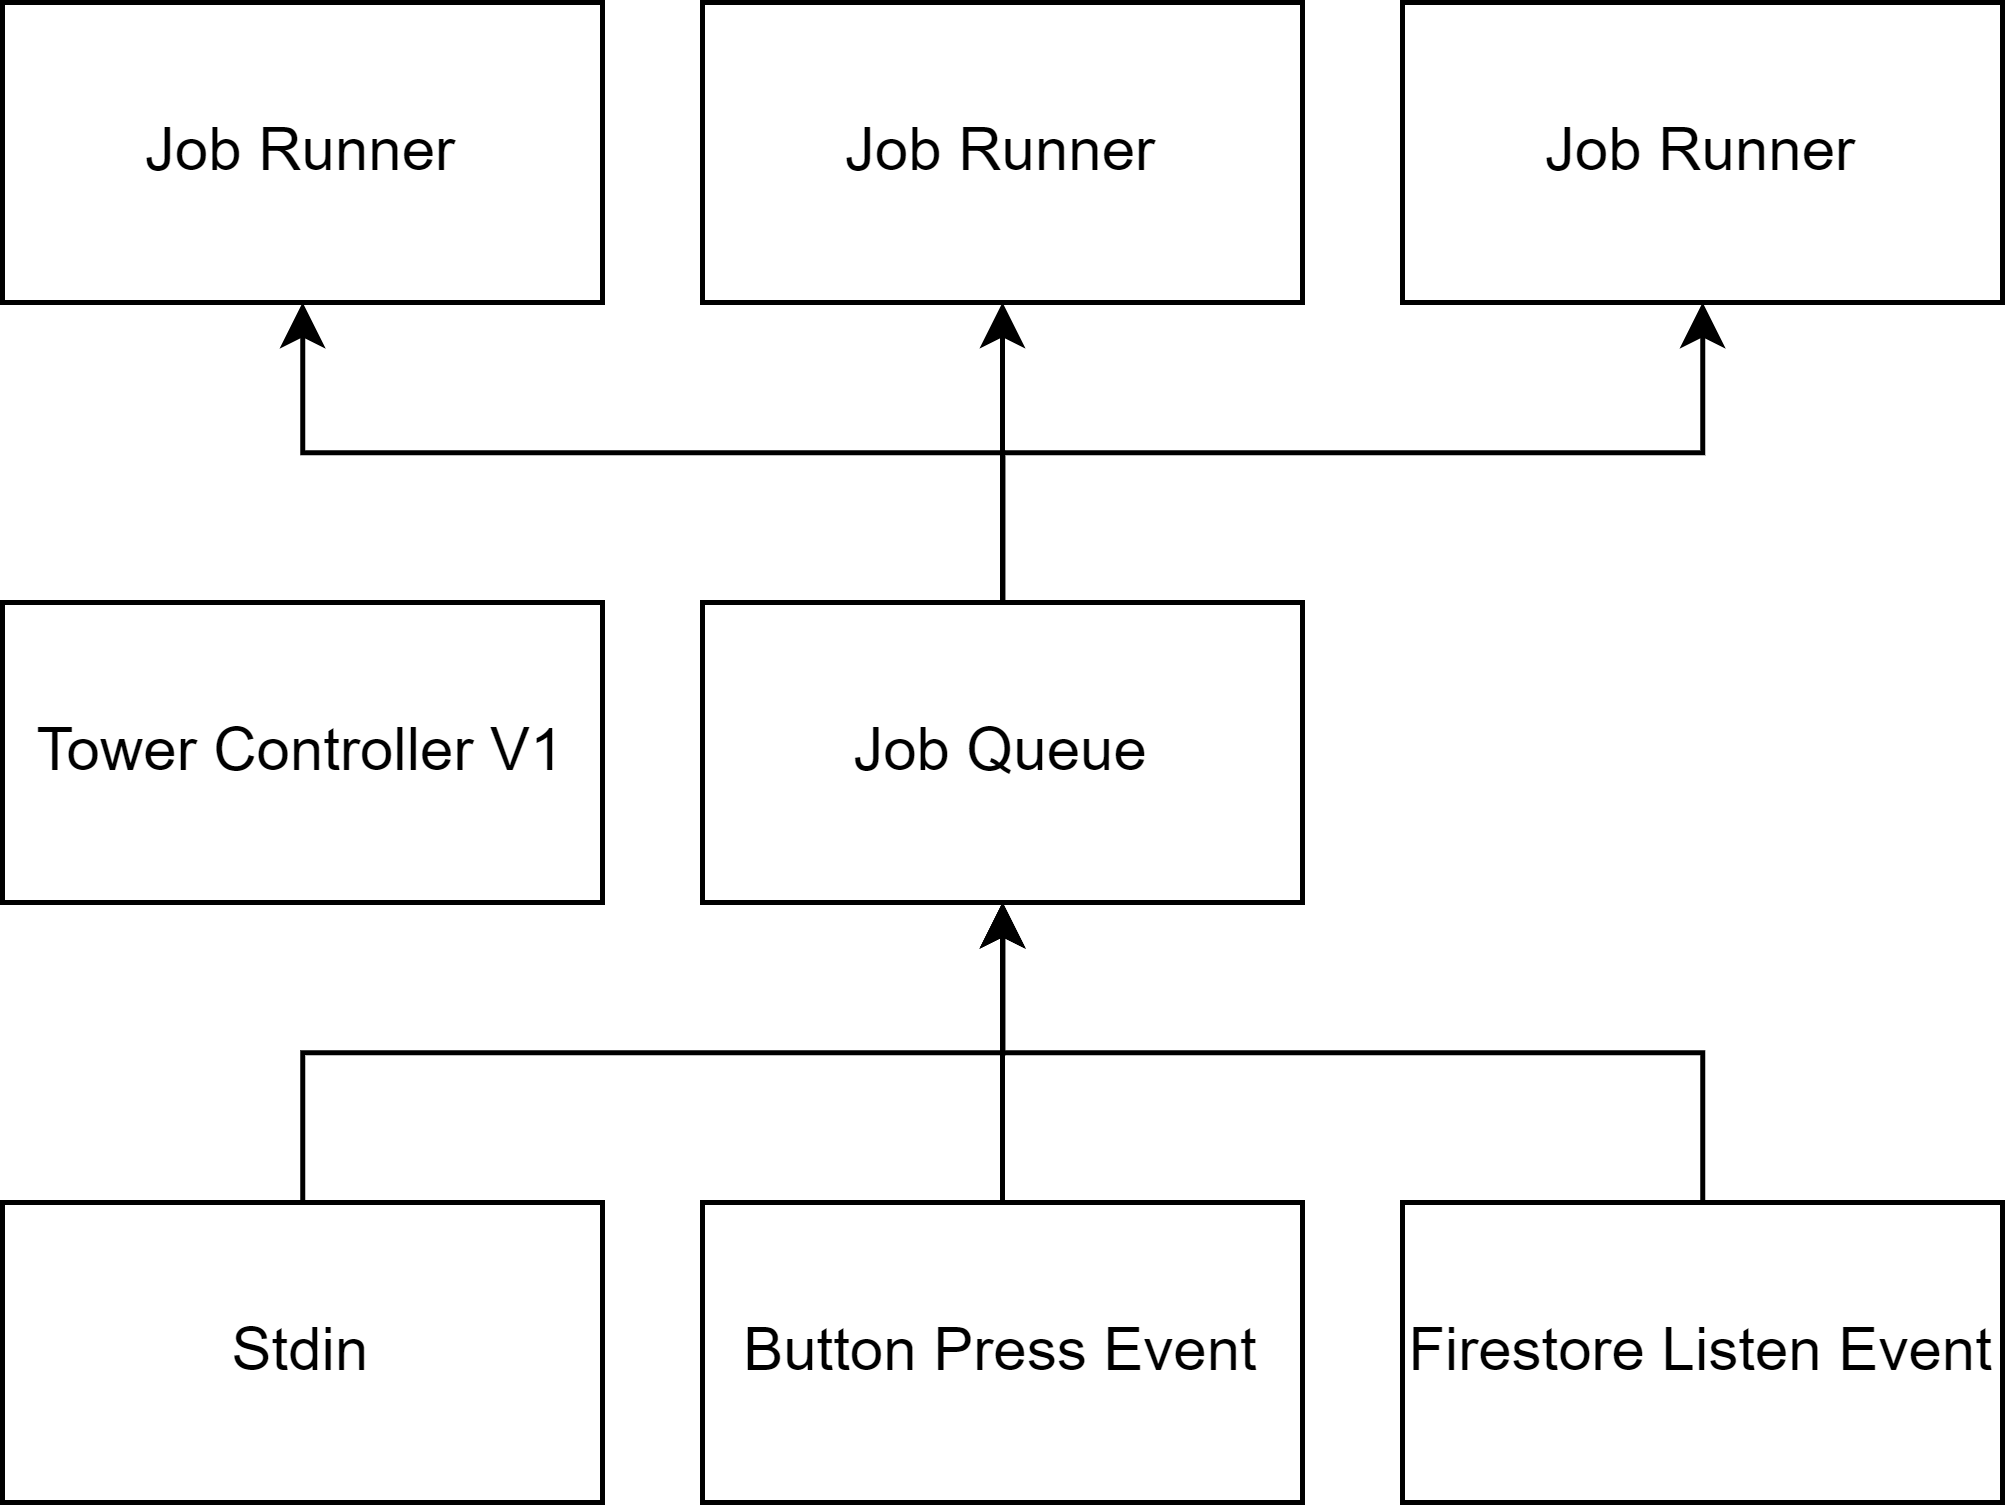
\includegraphics[width=0.5\textwidth]{images/tower_controller_v1.png}
  \caption{Datenströme des Tower Controller V1}
  \label{fig:tower_controller_v1}
\end{figure}

\ac{Stdin} und \ac{Stdout} werden verwendet um mit dem Benutzer zu kommunizieren. \ac{Stdin} wird verwendet, damit ein Benutzer manuell Jobs zur Queue hinzufügen kann. Dies ist vorallem bei zum \Gls{debuggen} nützlich. \ac{Stdout} wird verwendet um dem Benutzer Informationen über den aktuellen Status des Turms zu geben. Eingaben sind eine blockierende Operation, deshalb wurde aioconsole verwendet um \ac{Stdin} asynchron auszuführen.

In einem weiteren \Gls{thread} kommuniziert ein \ac{GPIO} \Gls{listener} mit einem physikalischen Button, welcher zur bestätigung des Einlagerungsvorgangs verwendet werden sollte. Der \Gls{listener} wartet auf einen Tastendruck und fügt anschließend einen Job (\Gls{event}) zur \Gls{queue} hinzu.

Der wichtigste \Gls{listener}ist der Datenbanklistener, dieser wartet auf Änderungen in der Datenbank und fügt entsprechende Jobs zur Queue hinzu. Dieser \Gls{listener} ist essenziell für die Kommunikation zwischen der App und dem Turm. Der \Gls{listener} wird von der offiziellen Python Bibliothek für Firebase bereitgestellt.

Zusätzlich wurde eine \ac{GUI} entwickelt, welche die aktuellen Zustände der einzelnen Radboxen darstellt. Diese \ac{GUI} wird ebenfalls von einem \Gls{thread} ausgeführt und aktualisiert sich automatisch, wenn sich der Zustand der Radboxen ändert. Die \ac{GUI} ist in tkinter implementiert und soll zu bei der Entwicklung helfen, falls das Programm nicht auf dem Raspberri Pi ausgeführt wird oder die Elektrotechnik noch nicht fertig ist.

Die Python Version war zu Anfang vielversprechend, jedoch gab es einige Probleme mit der Architektur, die zu einem komplizierten und unübersichtlichen Code führten. Die Architektur wurde in der V2 komplett überarbeitet.
